% !TEX TS-program = pdflatex
% !TeX program = pdflatex
% !TEX encoding = UTF-8 Unicode
% !TEX spellcheck = fr
\documentclass[]{beamer} %compress

\usepackage{amsmath,amssymb}             % AMS Math
\usepackage[T1]{fontenc}
\usepackage[utf8]{inputenc}
\usepackage[french,english]{babel}
\usepackage{txfonts} 
\usepackage[]{graphicx}
\usepackage{multirow}
\usepackage{hyperref}

\newcommand{\lien}[1]{{\tiny\url{#1}}}

%THEMES
%-------
%W/o navigation bar: default, boxes, Bergen, Madrid, Pittsburgh, Rochester
%With a treelike navigation bar: Antibes, JuanLesPins, Montpellier.
%With a TOC sidebar: Berkeley, PaloAlto, Goettingen, Marburg, Hannover
%With a mini frame navigation: Berlin, Ilmenau, Dresden, Darmstadt, Frankfurt, Singapore, Szeged
%With section and subsection titles: Copenhagen, Luebeck, Malmoe, Warsaw
\usetheme{Warsaw} % Antibes Boadilla Warsaw
%\usecolortheme{lily} % Beamer color theme
\usepackage{amsmath}

\title[Apprentissage automatique] %
{Apprentissage automatique}
\institute{}
\author[A. Aries]{\footnotesize Abdelkrime Aries}

\date{11 Décembre 2018}

\setbeamertemplate{navigation symbols}{%
	\usebeamerfont{footline}%
	\color{black}
	\normalsize
	\hspace{.5em}%
	\bfseries
	\insertframenumber/\inserttotalframenumber
}

\setbeamertemplate{headline}{}


\begin{document}

\begin{frame}
\maketitle
\end{frame}

%\begin{frame}
%\frametitle{Table of content}
%{\scriptsize
%\tableofcontents
%}
%\end{frame}

%==================================================
%==================================================
\section{Introduction}

\begin{frame}

\begin{center}
	\Huge\bfseries Introduction
\end{center}

\end{frame}

%-----------

\subsection{Motivation}

\begin{frame}
\frametitle{Motivation}

\begin{itemize}
	\item Certaines tâches sont difficiles à programmer manuellement: Reconnaissance de formes, Traduction par machine, Reconnaissance de la parole, Aide à la décision, etc.
	\item Les données sont disponibles, qui peuvent être utilisé pour estimer la fonction de notre tâche 
\end{itemize}

\end{frame}

%-----------

\subsection{Applications}

\begin{frame}
\frametitle{Applications}

\begin{itemize}
	\item Santé:
	\begin{itemize}
		\item Watson santé de IBM: \lien{https://www.ibm.com/watson/health/}
		\item Projet Hanover de Microsoft: \lien{https://hanover.azurewebsites.net}
		\item DeepMind santé de Google: \lien{https://deepmind.com/applied/deepmind-health/}
	\end{itemize}

	\item Finance \cite{2018-EISENBERG}: Prévention de fraude, management de risques, prédiction des investissements, etc.
	\item Domaine légal \cite{2017-beyer}: cas de CaseText \lien{https://casetext.com}
	\item Traduction: Google traslate \lien{https://translate.google.com/}
\end{itemize}

\end{frame}

%-----------

\subsection{Types des algorithmes}

\begin{frame}
\frametitle{Types des algorithmes}

\begin{itemize}
	\item Apprentissage Supervisé: Lorsque nous avons les données et leurs sorties.
	\item Apprentissage Non Supervisé: Lorsque nous avons les données seulement.
	\item Apprentissage par renforcement: Lorsque nous avons les données et une méthode pour mesurer la qualité des sorties sans savoir les sorties correctes. 
\end{itemize}

\end{frame}

%-----------

\begin{frame}
\frametitle{Apprentissage supervisé}


Classification 

Régression 

\end{frame}

%-----------

\begin{frame}
\frametitle{Apprentissage non supervisé}

Lorsque nous avons 

Classification 

Régression 

\end{frame}

%-----------

\begin{frame}
\frametitle{Apprentissage par renforcement} 

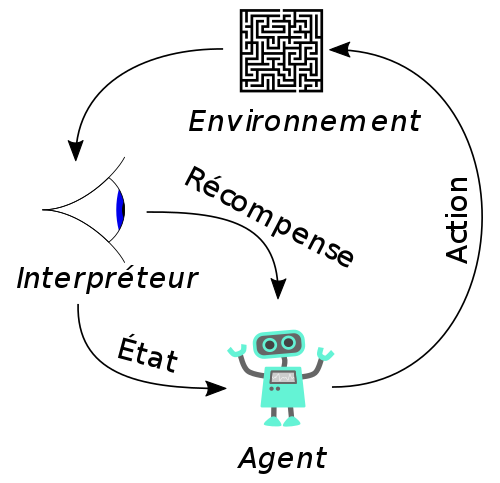
\includegraphics[height=\textheight]{../IMG/RL-fr.png}

\end{frame}

%-----------

\subsection{Limites}

\begin{frame}
\frametitle{Limites}

\end{frame}

%-----------

\subsection{Outils}

\begin{frame}
\frametitle{Outils}

\begin{tabular}{llll}
	Outil & Licence & Langage & Interface \\
	Deeplearning4j & Apache-2 & C++, Java & Java, Scala, Clojure, Python (Keras), Kotlin \\
\end{tabular}

\end{frame}

%-----------

\subsection{Évaluation}

\begin{frame}
\frametitle{Évaluation}

\end{frame}

% ==================================================
% ==================================================
\section{Préparation de données}

\begin{frame}

\begin{center}
	\Huge\bfseries Préparation de données
\end{center}

\end{frame}

\subsection{Construction de données}

\begin{frame}
\frametitle{Construction de données}

\begin{itemize}
\item 
\end{itemize}

\end{frame}

%++++++++++++++++++++++++++++++++++++++++++++++++++
%++++++++++++++++++++++++++++++++++++++++++++++++++
%++++++++++++++++++++++++++++++++++++++++++++++++++
\begin{frame}

\begin{center}
	\Huge\bfseries Apprentissage supervisé
\end{center}

\begin{itemize}
	\item Classification naïve bayésienne (Naive Bayes)
	\item Machine à vecteurs de support (SVM)
	\item Régression linéaire
	\item Régression logistique
	\item Perceptron
	\item Réseau de neurones artificiels
\end{itemize}

\end{frame}

%==================================================
%==================================================
\section{Classification naïve bayésienne}

\begin{frame}

\begin{center}
	\Huge\bfseries Classification naïve bayésienne
\end{center}

\end{frame}

%-----------

%==================================================
%==================================================
\section{Machine à vecteurs de support}

\begin{frame}

\begin{center}
	\Huge\bfseries Machine à vecteurs de support
\end{center}

\end{frame}

%-----------

%++++++++++++++++++++++++++++++++++++++++++++++++++
%++++++++++++++++++++++++++++++++++++++++++++++++++
\begin{frame}

\begin{center}
	\Huge\bfseries Apprentissage non supervisé
\end{center}

\begin{itemize}
	\item Regroupement K-Means
	\item Auto-encodeurs (Réseaux de neurones)
\end{itemize}

\end{frame}



\begin{frame}
\begin{center}
	\frametitle{Bibliographie}
	\scriptsize
	\bibliographystyle{apalike}
	\bibliography{cite}
\end{center}
\end{frame}

\end{document}

